\documentclass[french]{article}
\usepackage[utf8]{inputenc}
\usepackage[T1]{fontenc}
\usepackage{babel}
\usepackage{lmodern}
\usepackage{graphicx}
\usepackage{tikz}
\usepackage{fullpage}

\usepackage{amsmath}
\usepackage{amsfonts}

\title{Algorithmique 2}
\date{}
\author{L3 RI}


\begin{document}
\maketitle
\tableofcontents

\section{NP-Complétude}

\begin{center}
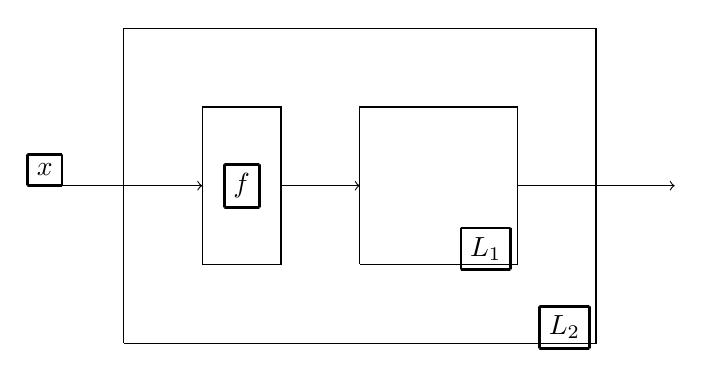
\begin{tikzpicture}
\draw (1,0) -- (1,4) -- (7,4) -- (7,0) -- (1,0);
\draw (2,1) -- (2,3) -- (3,3) -- (3,1) -- (2,1);
\draw (4,1) -- (4,3) -- (6,3) -- (6,1) -- (4,1);
\draw[->] (0,2) -- (2,2);
\draw[->] (3,2) -- (4,2);
\draw[->] (6,2) -- (8,2);
\node[draw,line width=-1] at (0,2.2) {$x$};
\node[draw,line width=-1] at (2.5,2) {$f$};
\node[draw,line width=-1] at (5.6,1.2) {$L_1$};
\node[draw,line width=-1] at (6.6,0.2) {$L_2$};
\end{tikzpicture}
\end{center}

\section{Algorithmes d'approximation}

\section{Algorithmes probabilistes}

\section{Géométrie algorithmique}

\section{Algorithmes distribués}



\end{document}
